\subsection{Ergebnisse}
Das Kapitel der Ergebnisse befasst sich mit der konkreten Umsetzung der Xamarin Applikation und dem PlayFramework. Wir haben uns dabei ganz konkret für die nachfolgenden Code-Beispiele entschieden. Der Grund dafür ist, dass diese entweder den typischen Aufbau einer Methode zeigen oder wie das Listing \ref{watcher}, eine Kernlogik darstellen. 
Bei den Ergebnissen der Xamarin App zeigen wir zusätzlich noch eine kurze Retrospektive auf geplantes Design und effektiver Umsetzung des GUIs. Das Kapitel wird durch eine Gegenüberstellung der erreichten und geplanten Arbeit abgeschlossen.

Zur besseren Übersicht wurde der Code vereinzelt gekürzt. Dies ist durch 3 Punkte (...) gekennzeichnet.

\subsubsection{Implementierung des PlayFrameworks}
Die Umsetzung des Backends basiert auf dem PlayFramework. Die Gründe für diesen Entscheid können in Kapitel \ref{vorstudie} nachgelesen werden. 

Um die Daten permanent zu speichern, besitzt das PlayFramework eine Anbindung an eine MongoDB Instanz. Die Anbindung wurde mit dem MongoDB Async Driver für Java \cite{MongoDBAsyncDriver} realisiert. Die Implementation ist daher auch in Java geschrieben. Für die Dokumentation des Backends verwendeten wir Swagger \cite{swagger}.

\paragraph*{ParticipantController.java}
Die nachfolgenden Listings zeigen einen Ausschnitt aus der \texttt{ParticipantController.java} Klasse. Diese befindet sich in der LogicComponent (Abbildung \ref{fig:architektur-methode635}) vom PlayFramework.

\lstset{language=JAVA, showstringspaces=false, frame=single, captionpos=b, label=createParticipant, breaklines=true, numbers=left}
\begin{lstlisting}[caption={Participant erstellen}, label=participantErstellen]
public Result createParticipant(){

    JsonNode body = request().body().asJson();

    if (body == null ) {
        return forbidden(Json.toJson(new ErrorMessage("Error", "json body is null")));
    } else if(  body.hasNonNull("username") &&
            	body.hasNonNull("password") &&
            	body.hasNonNull("firstname") &&
            	body.hasNonNull("lastname")) {

    Participant participant = new Participant(body.get("username").asText(), body.get("password").asText(), body.get("firstname").asText(), body.get("lastname").asText());

    participantCollection.insertOne(participant, new SingleResultCallback<Void>() {
        @Override
        public void onResult(Void result, Throwable t) {
            Logger.info("Inserted Participant!");
        }
    });

    return ok(Json.toJson(new SuccessMessage("Success", "Participant successfully inserted")));
    }

    return forbidden(Json.toJson(new ErrorMessage("Error", "json body not as expected")));
}
\end{lstlisting}

Bei der Methode für das Erstellen von Participants, prüft das Framework zuerst, ob ein HTML-Body existiert. Ist dies nicht der Fall, sendet es ein HTTP-Response Status-Code (Zeile 24) zurück.

Existiert ein HTML-Body, wird dieser auf die Existenz der Felder \textit{username}, \textit{password}, \textit{firstname} und \textit{lastname} geprüft (Zeile 7-10). Daraus erstellt das Framework als nächstes ein \texttt{participant} (Zeile 12), welcher mittels  \texttt{insertOne} in die \texttt{participant\-Collection} gespeichert wird (Zeile 14).

Zuletzt sendet das PlayFramework eine Antwort mit dem HTTP-Status Code 200 und einer Nachricht an den Absender. 

\begin{lstlisting}[caption={Login}]
public Result login() throws UnsupportedEncodingException, ExecutionException, InterruptedException {
...
if (body.hasNonNull("username") && body.hasNonNull("password")) {
    CompletableFuture<Participant> future = new CompletableFuture<>();

    participantCollection.find(and(
    eq("username", body.get("username").asText()),
    eq("password", body.get("password").asText()))).first(new SingleResultCallback<Participant>() {
        @Override
        public void onResult(Participant participant, Throwable t) {
            if (participant != null) {
                Logger.info("Found participant");
                future.complete(participant);
            } else {
                future.complete(null);
            }
        }
    });

    if (future.get()!= null){
        ObjectNode result = Json.newObject();
        result.putPOJO("participant", future.get());
        result.put("access_token", getSignedToken(7l));
        return ok(result);
    } else {...}
} else {...}
}
\end{lstlisting}

Für das Login eines Participants schaut auch hier zuerst das Framework im HTML-Body nach der Existenz der Felder \textit{username} und \textit{password} (Zeile 3). Im nächsten Schritt durchsucht es die Datenbank nach einem Participant mit den angegebenen Werten (Zeile 6-8). 

Da wir einen asynchronen Treiber verwenden, benötigen wir ein \texttt{CompletableFuture}, um das Resultat der Abfrage darin abzuspeichern und um mittels \texttt{future.get()} darauf zugreifen zu können (Zeile 20).

Am Ende wird dem Resultat neben dem gefundenen \textit{participant} noch ein \textit{JWT-Token} angefügt (Zeile 21-24).

\paragraph*{TeamController.java}
Das Listing \ref{teamBeitreten} zeigt einen Ausschnitt aus der \texttt{TeamController.java} Klasse. Auch diese befindet sich in der LogicComponent (Abbildung \ref{fig:architektur-methode635}) vom PlayFramework.
\begin{lstlisting}[caption={Einem Team beitreten}, label=teamBeitreten]
public Result joinBrainstormingTeam(String teamIdentifier) throws ExecutionException, InterruptedException {
...
if (brainstormingTeam!= null && brainstormingTeam.getNrOfParticipants() > brainstormingTeam.getCurrentNrOfParticipants() && brainstormingTeam.joinTeam(participant)) {

    teamCollection.updateOne(eq("identifier", teamIdentifier),combine(set("participants", brainstormingTeam.getParticipants()), inc("currentNrOfParticipants", 1)), new SingleResultCallback<UpdateResult>() {
        @Override
        public void onResult(final UpdateResult result, final Throwable t) {
            Logger.info(result.getModifiedCount() + " Team successfully updated");
        }
    });

    return ok(Json.toJson(new SuccessMessage("Success", "Participant successfully added to the brainstormingTeam")));

} else {
    ...
}
...
}
\end{lstlisting}

Dieses Beispiel soll zeigen, wie mit dem MongoDB Async Driver ein Eintrag mittels \texttt{updateOne} aktualisiert werden kann.

Wie auch schon bei der \texttt{find} Methode, kennzeichnet der erste Parameter das Dokument, welches man aktualisieren möchte. Der zweite Parameter steht für die Felder und deren neuen Werte und der dritte und letzte Parameter ist wieder der \texttt{SingleResultCallback} und beschreibt wie das Resultat weiter prozessiert wird. All dies ist auf Zeile 5-8 zu finden.

\paragraph*{FindingController.java}
Das Listing \ref{watcher} zeigt einen Ausschnitt aus der \texttt{FindingController.java} Klasse. Wie auch schon die vorherigen Klassen, befindet sich auch diese in der LogicComponent (Abbildung \ref{fig:architektur-methode635}) vom PlayFramework.
\begin{lstlisting}[caption={Watcher für BrainstormingFinding}, label=watcher]
private void startWatcherForBrainstormingFinding(String identifier){

ScheduledExecutorService executor = Executors.newSingleThreadScheduledExecutor();

TimerTask task = new TimerTask() {
    @Override
    public void run() {
        try {
    	...
	if (finding.getCurrentRound() > finding.getBrainsheets().size()){
	    lastRound(identifier);
	    executor.shutdown();
	}

	if (endDateTime.plusSeconds(30).isBeforeNow() ||
	finding.getDeliveredBrainsheetsInCurrentRound() >= finding.getBrainsheets().size()){
	nextRound(identifier);
	}
            cancel();

        } catch (ExecutionException e) {
            e.printStackTrace();
        } catch (InterruptedException e) {
            e.printStackTrace();
        }
    }
};

executor.scheduleAtFixedRate(task, 1000L, 5000L, TimeUnit.MILLISECONDS);
}
\end{lstlisting}

Um den Zustand über die verbleibende Zeit oder die bereits eingereichten \textit{Brainsheets} überwachen zu können, setzen wir einen \texttt{ScheduledExecutorService} \cite{JavaTimer} ein. Dieser erlaubt uns alle 5000ms bzw. alle 5s den \texttt{TimerTask} auf Zeile 5 auszuführen. 

Der \texttt{TimerTask} prüft zuerst, ob die aktuelle Runde schon die letzte Runde ist (Zeile 10). Ist dies der Fall, führt er die Methode \textit{lastRound(identifier)} aus und beendet den executor, sodass keine neuen \texttt{TimerTask} Objekte gestartet werden. In diesem Zustand ist das gesamte \textit{BrainstormingFinding} ausgefüllt.

Ist dies nicht der Fall, prüft er als nächstes, ob die Endzeit der aktuellen Runde plus 30s noch vor der aktuellen Uhrzeit liegt (Zeile 15). Die Bedingung auf Zeile 16 prüft, ob alle \textit{Brainsheets}, welche für die Abgabe erwartet werden schon abgegeben wurden. Unabhängig welche dieser zwei Bedingungen (Zeile 15 oder 16) zuerst eintrifft, es wird anschliessend immer die Methode \textit{nextRound(identifier)} ausgeführt.

Sollte keine der Bedingungen (Zeile 10, 15 oder 16) zutreffen, so beendet sich der \texttt{TimerTask} mittels \textit{cancel} selbst. 

Da der executor aber nach 5s den nächsten \texttt{TimerTask} startet, ist so für die gesamte Dauer, für die das \textit{BrainstormingFinding} läuft, ein 'Watcher' für den korrekten Ablauf zuständig. Die Methode \textit{startWatcherForBrainstormingFinding(String identifier)} wird beim Start eines \textit{BrainstormingFinding} ausgeführt.

\begin{lstlisting}
public Result startBrainstorming(String findingIdentifer) throws ExecutionException, InterruptedException {
        startWatcherForBrainstormingFinding(findingIdentifer);
        return nextRound(findingIdentifer);
}
\end{lstlisting}

\subsubsection{Implementierung der Xamarin App}
Um ein sauberes Design des Frontends zu ermöglichen, ist das MVVM\--Framework Prism.Forms \cite{prism} im Einsatz. Dies vereinfacht die Verwendung des MVVM-Patterns, das bei Xamarin üblich ist und die Views von dessen ViewModels abkapselt. Die ViewModels werden mit diesem Framework entweder per Konvention oder per Konfiguration miteinander verknüpft, sodass der \texttt{BindingContext} einer View auf das entsprechende ViewModel gesetzt ist. Dieser wird benötigt, um die berechneten Werte der Variablen im User Interface darzustellen. In Listing \ref{register-vm} verknüpfen wir das MainPageViewModel mit der MainPageView, sodass wir darauf navigieren können. 

\begin{lstlisting}[label=register-vm,caption=Verknüpfung von View mit ViewModel in Prism.Forms]
containerRegistry.RegisterForNavigation<MainPage, MainPageViewModel>();
\end{lstlisting}

Das Framework bietet weiter \textit{Dependency Injection} an. Zum Beispiel kann so ein Navigation Service jeder Komponente im Konstruktor mitgegeben werden, dass diesem das Navigieren ermöglicht wird. 

Als Ausgangslage für die Umsetzung dienten die Mockups. Aufgrund diesen recherchierten wir in der Dokumentation von Xamarin Forms nach möglichen User Controls und Layouts, die eingesetzt werden sollten. Dabei stellte sich heraus, dass das erarbeitete Navigationskonzept in den Mockups sich nicht implementieren liess. Problem dabei war, dass das Mockup mit den von Xamarin Forms dargebotenen Layouts nur sehr umständlich programmiert werden konnte. Dabei hätten wir eine \texttt{MasterDetailPage} mit Swipe Gestures erweitern müssen, welche aber schon vom Framework für einen anderen Zweck verwendet werden. Deshalb haben wir uns für eine \texttt{TabbedPage} entschieden, die die relevanten Daten ebenso nützlich darstellt. In Abbildung \ref{fig:comparison-mockup-app} sind die Unterschiede zwischen  der App und dem Mockup ersichtlich.

\begin{figure}
	\centering
	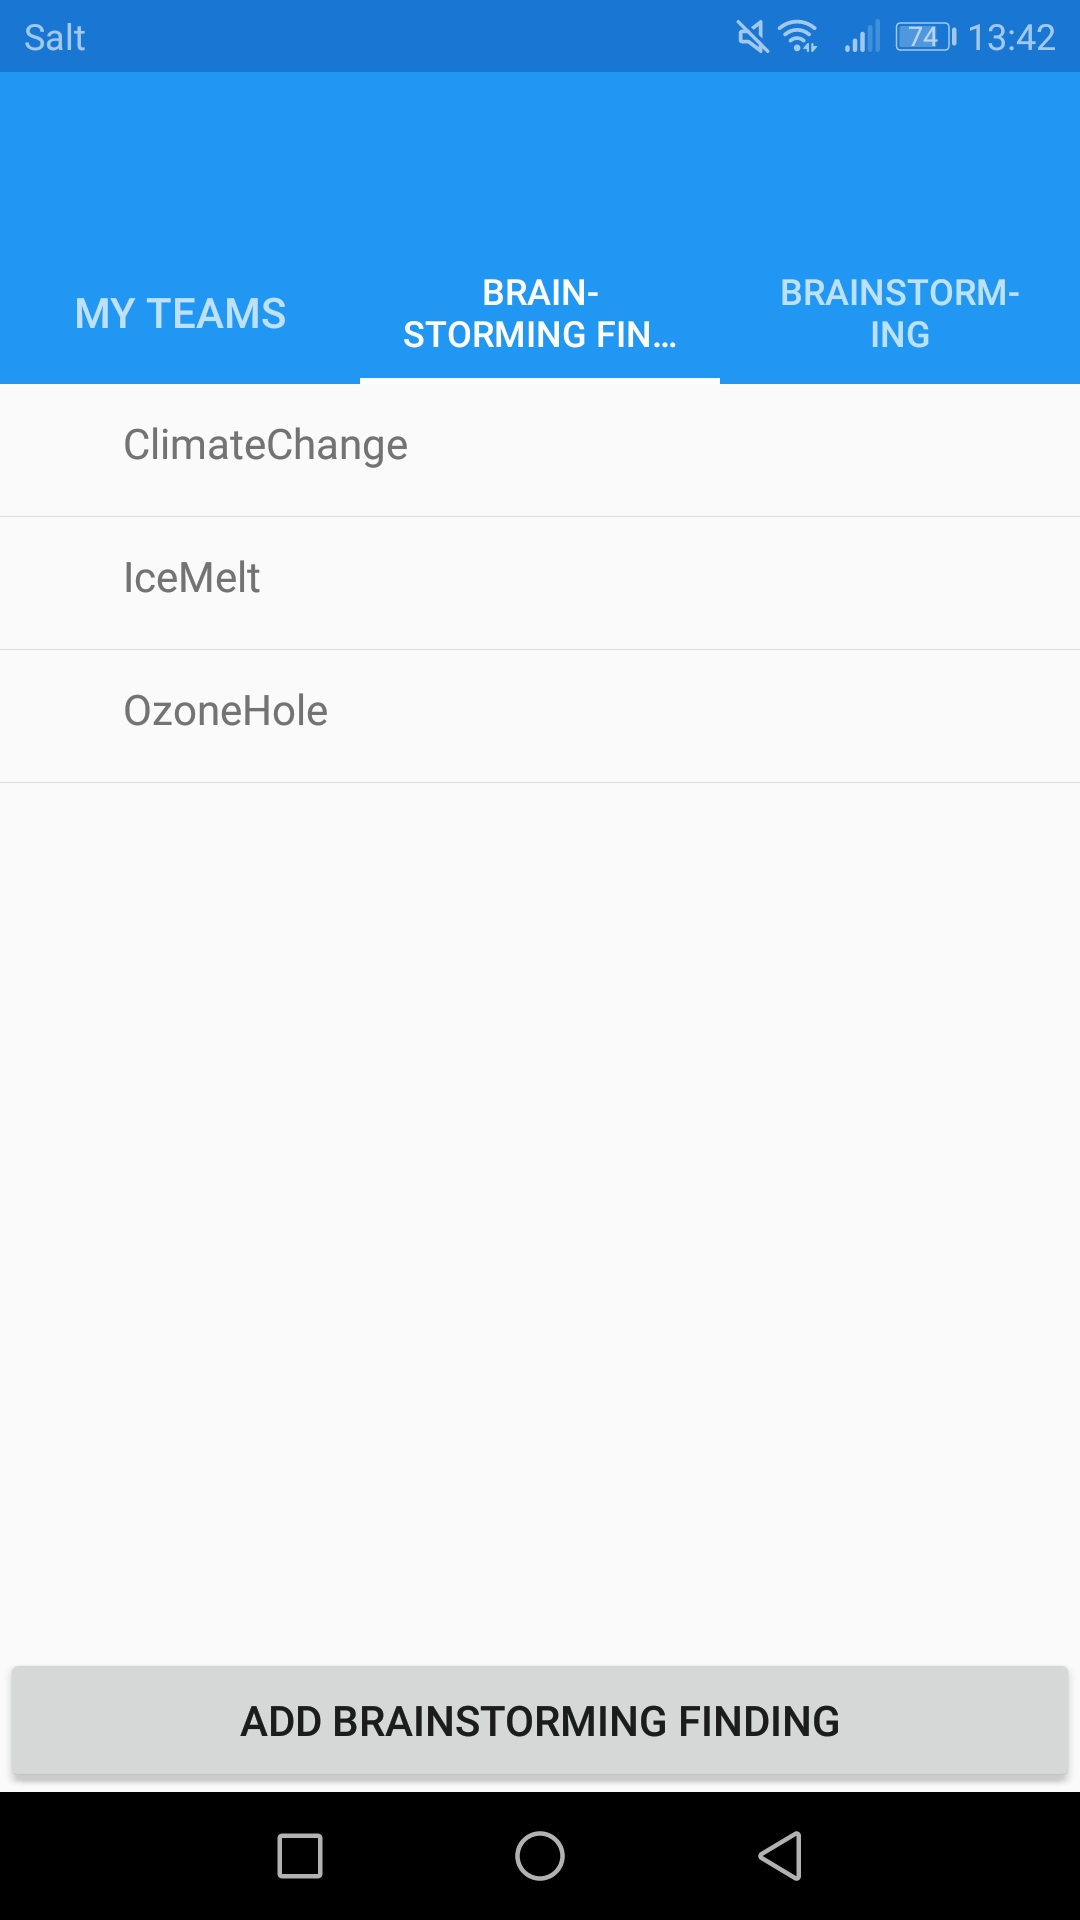
\includegraphics[width=0.4\linewidth, height=0.45\textheight]{img/techn-bericht/finding-list_app}
	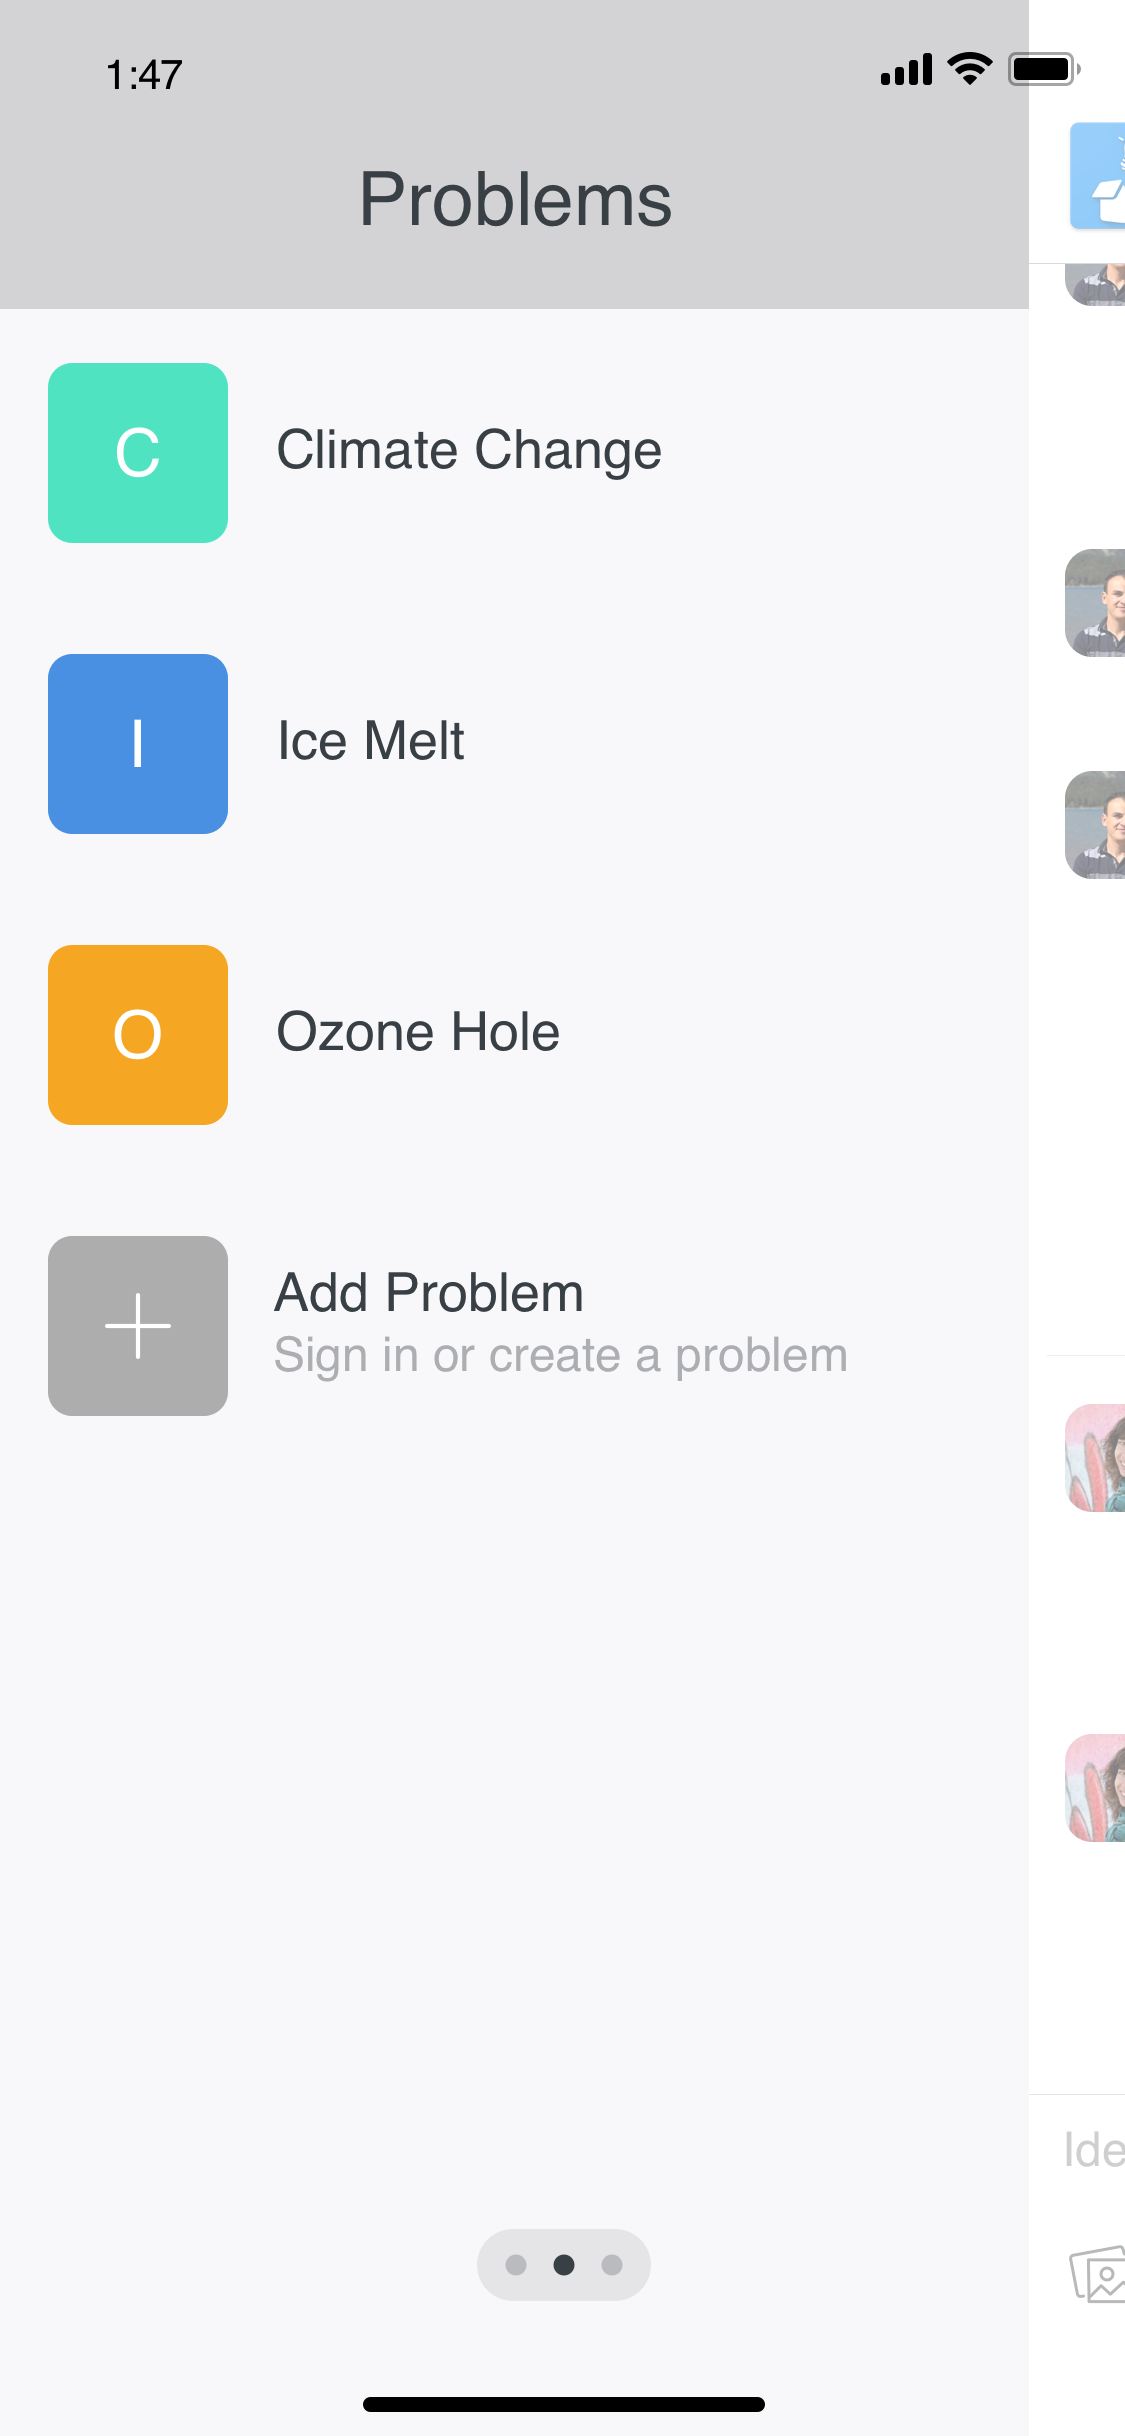
\includegraphics[width=0.4\linewidth, height=0.45\textheight]{img/techn-bericht/finding-list_mockup}
	\caption{Vergleich App und Mockup}
	\label{fig:comparison-mockup-app}
\end{figure}
	
\paragraph*{Umsetzung Brainstorming}
Die Brainstorming Page besteht aus drei visuellen Bereichen, dem Header, Footer und Center. Je nach Zustand des BrainstormingFindings werden Elemente davon angezeigt oder nicht. Es gibt 3 Zustände, indem ein Brainstorming sein kann:
\begin{enumerate}
	\item \textbf{Waiting}. Das Brainstorming ist erstellt und es wird darauf gewartet, dass der Moderator den Prozess startet.
	\item \textbf{Running}. Das Brainstorming läuft und die Runden werden herauf- und die verbleibende Zeit pro Runde heruntergezählt.
	\item \textbf{Ended}. Das Brainstorming ist beendet.
\end{enumerate}
Tabelle \ref{tab:visual-elements} zeigt die Sichtbarkeit einiger relevanten Controls im Brainstorming.

\renewcommand{\arraystretch}{1.5}
\begin{center}
	\begin{longtable}{| l | p{2cm} |p{2cm} |p{2cm} |}
		
		\hline
		&Waiting & Running & Ended\\
		\hline
		\textbf{Header}	& & & \\
		Send Button & \checkmark (disabled) & \checkmark & x\\
		RemainingTime & \checkmark (00m:00s) & \checkmark & x\\
		'Completed' & x & x & \checkmark\\
		\hline
		\textbf{Center}	& & & \\
		BrainSheets & x & \checkmark & \checkmark\\
		\hline
		\textbf{Footer}	& & & \\
		Commit Button & \checkmark (disabled) & \checkmark & x\\
		Text Entry & \checkmark & \checkmark & x\\
		\hline
		\caption{Sichtbarkeit nach Zustände im Brainstorming}

		\label{tab:visual-elements}
	\end{longtable}
\end{center}


Einige der erwähnten Komponenten können der Abbildung \ref{fig:brainstorming-overview} entnommen werden.



Für das Abfragen der verbleibenden Zeit in der aktuellen Runde ist ein \texttt{System.{\-}Timers.Timer} implementiert, der im Sekundentakt das Backend abfragt. Sinkt diese Zahl unter eine Sekunde, werden die vorhandenen Ideen der aktuellen BrainWave ans Backend gesendet. Gleichzeitig startet ein zusätzlicher Timer, der das BrainstormingFinding im Takt von 2.5s abfragt und prüft, ob sich die Runde geändert hat. Ist dies der Fall, müssen die betroffenen UI-Elemente aktualisiert werden. Die Logik, die vom zusätzlichen Timer aufgerufen wird, ist in der Methode \textit{UpdateRound()} im Listing \ref{Update-Round} zu finden.


\begin{lstlisting}[label=Update-Round,caption=Poll-Mechanismus um zu prüfen ob Runde gewechselt hat]
private void UpdateRound()
{
var backendFinding = _brainstormingFindingRestResolver.GetFinding(_context.CurrentFinding);
if (backendFinding.CurrentRound != _context.CurrentFinding.CurrentRound)
{
_context.CurrentFinding = backendFinding;
Console.WriteLine("Round has changed, proceeding to next round");
NextRound();
}
}
\end{lstlisting}

\begin{figure}
	\centering
	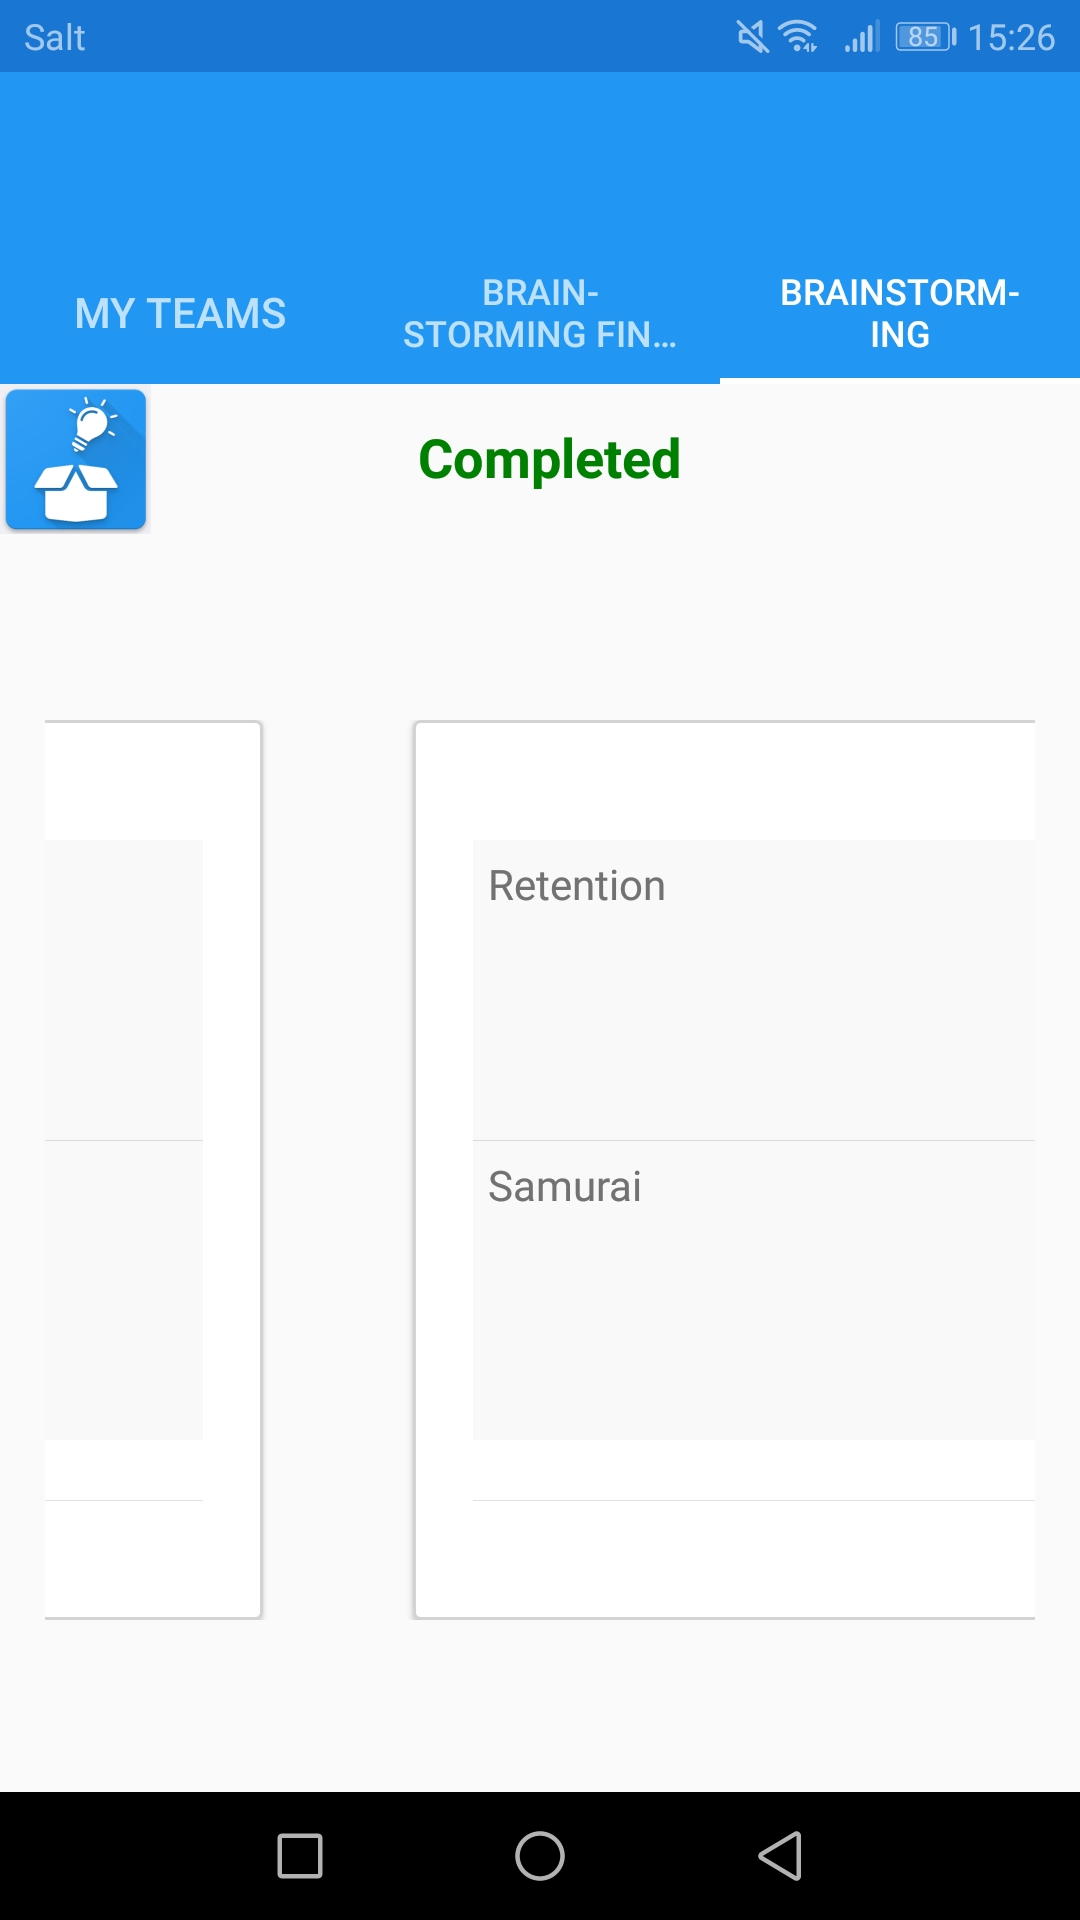
\includegraphics[width=0.4\linewidth,height=0.4\textheight,keepaspectratio]{img/techn-bericht/brainstorming-overview}
	\caption{Brainstorming Finding Übersicht während dem Swipen vom einen ins nächste BrainSheet}
	\label{fig:brainstorming-overview}
\end{figure}

\paragraph*{Create/Join Group mit QR-Code}
Wie in UC 10: Create Brainstorming Team und UC 5: Join Brainstorming Team spezifiziert, muss unser System einen Mechanismus für das Erstellen von Teams und beitreten in diese Teams bieten. 

Wir kreierten eine Lösung, die beim Erstellen des Teams einen QR-Code generiert, welcher von anderen Teammitgliedern mittels QR-Scanner einlesen werden kann. Durch den Scan-Vorgang treten die Mitglieder automatisch der erstellten Gruppe bei.

Um diesen Mechanismus umzusetzen, wurde eine Library namens ZXing \cite{zxing.net} verwendet, die wir im Rahmen der Recherche (Kapitel \ref{subsubsec:forms-vs-native}) entdeckten. Diese erlaubt es, ein Xamarin Control für das Scannen und das Generieren zu verwenden. Mit etwas plattform-spezifischem Konfigurationsaufwand funktioniert diese Library wie gewünscht.

Listing \ref{generate} demonstriert, wie das Generieren und Darstellen des QR-Codes in XAML funktioniert.


\begin{lstlisting}[label=generate,caption=Verwendung der ZXing Library fürs Generieren des QR-Codes]
<forms:ZXingBarcodeImageView BarcodeValue="{Binding Text}"  BarcodeFormat="QR_CODE">
\end{lstlisting}


Listing \ref{scan} zeigt das Gegenstück zum oben genannten Generieren, nämlich den XAML-Code, der für das Scannen verwendet wird. Der interessante Teil dabei ist das Property \texttt{ScanResultCommand}, was es mittels MVVM erlaubt, über einen Command eine parametrisierte Methode aufzurufen. Auf dem Parameter ist das Scan-Resultat als Text gespeichert. In unserem Fall entspricht dieser der Team-Id, aufgrund welcher der QR-Code generiert wurde. Die Team-Id wird danach verwendet, um mittels RESTful HTTP auf dem Backend den JoinTeam Endpoint aufzurufen, der wiederum den entsprechenden Eintrag in der Datenbank durchführt und somit den User ins Team einfügt.


\begin{lstlisting}[label=scan,caption=XAML fürs Scannen von QR-Codes]
<zxing:ZXingScannerView IsScanning="true" Options="{Binding BarcodeOptions}" WidthRequest="200" HeightRequest="200" ScanResultCommand="{Binding FoundTeamIdCommand}" />
<zxing:ZXingDefaultOverlay TopText="Place the code inside the area" Opacity="0.9" BottomText="{Binding BottomOverlayText}" />
\end{lstlisting}

Die Abbildung \ref{fig:scan-generate} zeigt die beiden Controls in Aktion. 

\begin{figure}
	\centering	
\includegraphics[width=0.4\linewidth,height=0.4\textheight,keepaspectratio]{img/techn-bericht/generate-view}
	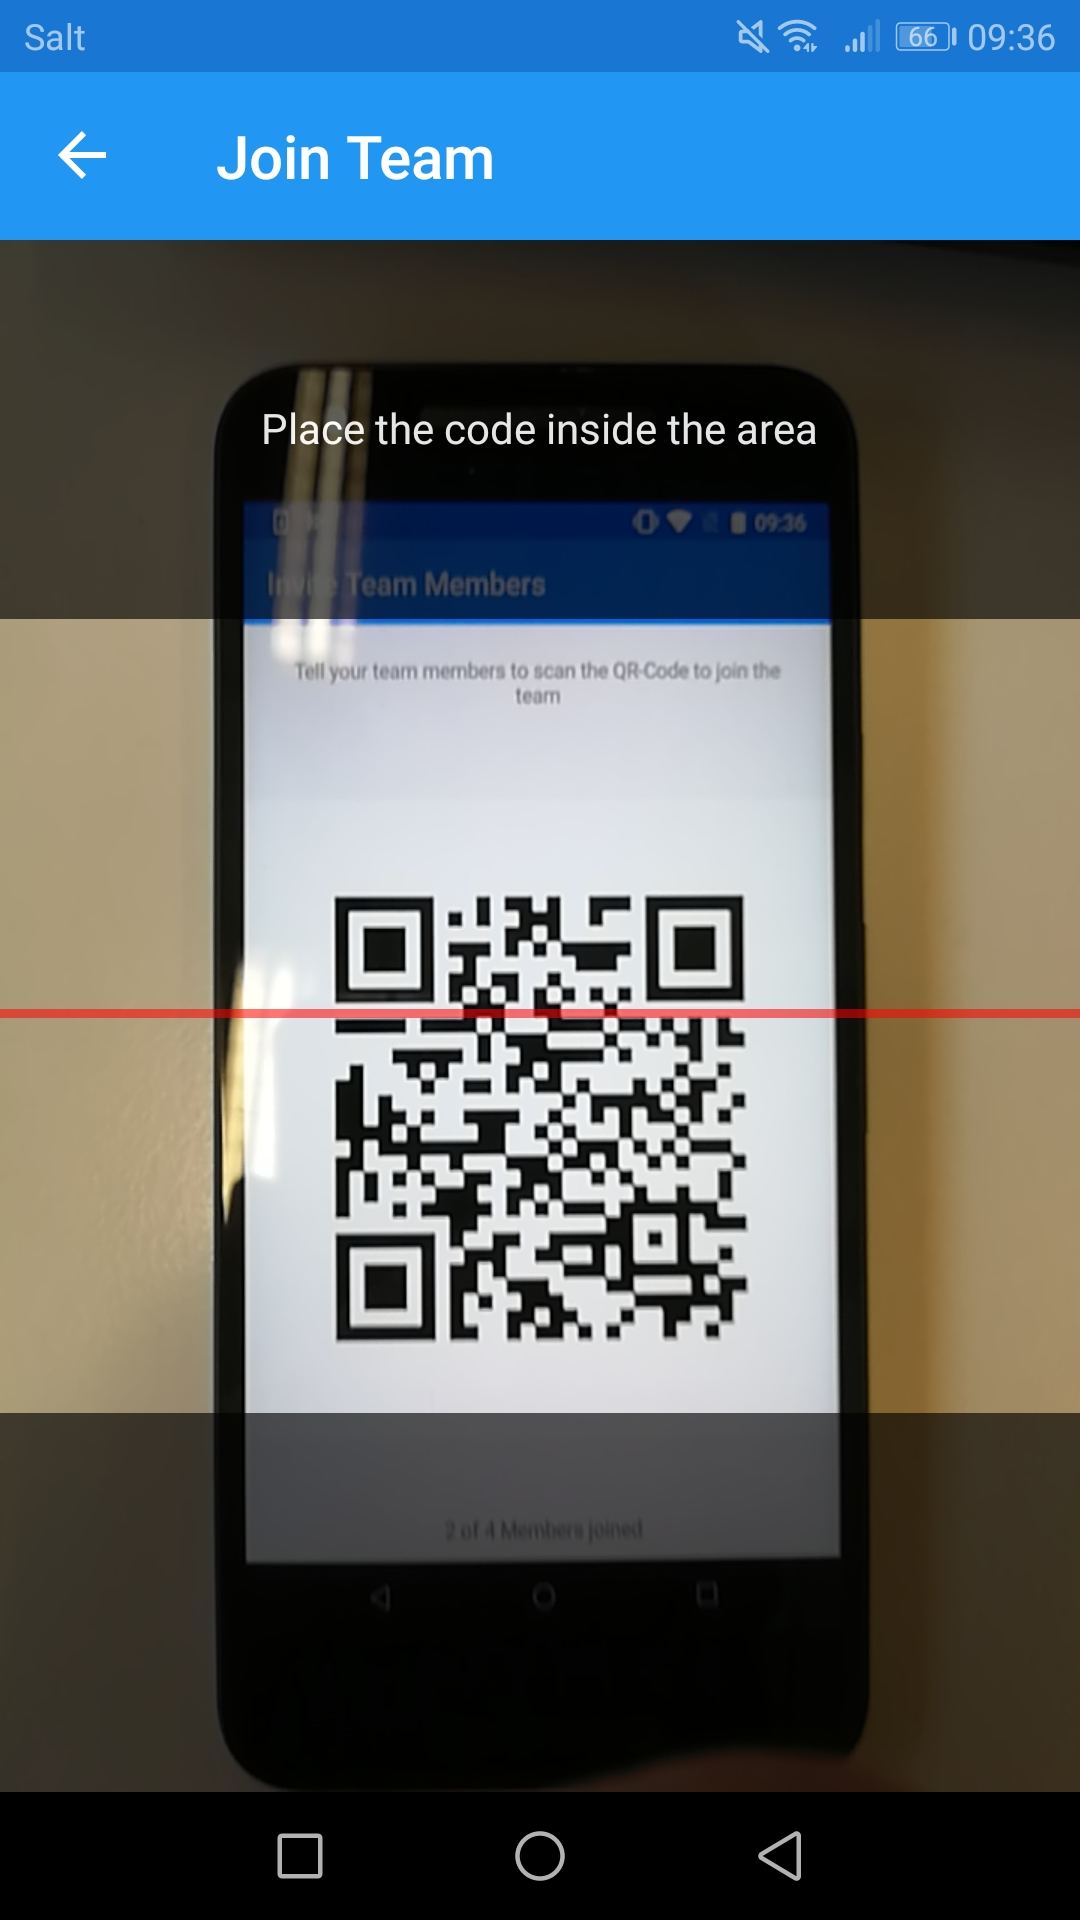
\includegraphics[width=0.4\linewidth,height=0.4\textheight,keepaspectratio]{img/techn-bericht/scan-view}
	\caption{Generierter QR-Code links und QR-Code Scan rechts}
	\label{fig:scan-generate}
\end{figure}

\subsubsection{Vergleich Soll/Ist}
Im Rückblick auf die in Kapitel \ref{subsec:ziele} formulierten Ziele und Liefergegenstände wurden die meisten Ziele erreicht. Die Konfigurierbarkeit ist durch die Applikation gegeben. Es ist daher möglich, Bestandteil von verschiedenen Teams zu sein und darin mehrere BrainstormingFindings mit unterschiedlichen Anzahl an Runden bzw. Zeit pro Runde zu erstellen. Des Weiteren werden Smartphone Fähigkeiten wie Kamera verwendet, um dem Team beizutreten. Hier sehen wir vor allem in Kombination mit der Erweiterbarkeit noch Potential, die Kamera als Mittel fürs Brainstorming selbst einzusetzen (gemäss UC8b: Insert Picture). Dass dies nicht dazu kam , liegt an der begrenzten Zeit von 14 Wochen. Aus gleichem Grund wurden die beiden anderen Sub-Use-Cases UC8a: Insert Weblink und UC8c: Insert Sketch nicht umgesetzt.

Das Persistieren von Ideen in unserem System bietet der Papierversion gegenüber einen Vorteil, da die einzige Information für das spätere Abholen der Ideen die Login-Daten sind. Mit diesen können alle jemals erfassten BrainstormingFindings wieder gelesen werden, während in der Papierversion die Unterlagen physisch hervorgeholt werden müssten, falls sie überhaupt archiviert wurden.  

Ein knapp erfülltes Ziel ist die Robustheit und Bedienbarkeit. So ist es ohne Weiteres möglich, die App gemäss ihrem Sinne auszuführen und zu verwenden, jedoch ist die Benutzerführung nicht überall intuitiv. Auch kann es vorkommen, dass ab und an ein Refresh benötigt wird. Zum Beispiel kann es sein, dass beim Starten des Brainstormings nicht bei allen Participants das entsprechende Sheet vorliegt, sondern die View leer bleibt. Dies hängt mit den in Kapitel \ref{subsub:design-issue} erläuterten Problemen zusammen und kann durch das Betätigen der Sync-Funktionlität auf dem Icon behoben werden. 

Weitere nicht implementierte Features sind UC 2: Logout auf Back- und Frontend sowie UC4: Delete Account und UC6: Leave Brainstorming Team auf dem Frontend. Da diese keine kritischen Erfolgsfaktoren sind und zur Kernfunktionlität nicht wesentlich beitragen, wurden diese nach iterativer Planung und Abwägen der Ressourcen nicht implementiert.

Ansonsten konnten alle spezifizierten Use-Cases komplett umgesetzt werden.